\chapter{Theoretische Grundlagen}
\label{cha:Grundlagen}
In diesem Kapitel werden Theoretische Grundlagen geschaffen, die zum weiteren Verständnis der Arbeit benötigt werden. Zuerst werden ausgewählte Video-Schnittstellen erläutert und verglichen und bewertet welchen praktischen Nutzen diese für handelsübliche embedded Linuxsysteme bietet. Im Weiteren werden zwei Linux Boards verglichen und bewertet sowie deren praktische Einsatzgebiete beispielhaft dargelegt.

\section{Video-Schnittstellen}
Unter Video-Schnittstellen kann man die Schnittstellen verstehen, die direkt zur Anzeige von Bilddaten dienen und physikalisch mit einer Anzeigeeinheit verbunden sind. Hier können sowohl Hardware- als auch Softwarekomponenten enthalten sein.
\subsection{VGA}
Unter VGA versteht man Video Graphics Array und wurde 1987 von IBM entwickelt. Der Stecker hat 15 Pins und liefert neben analogen Farbinformationen Horizontale und Vertikale Synchronisationssignale. Aufgrund der limitierten Spezifikationen ist die Schnittstelle eher antik und selbst Intel als Chiphersteller will ab 2015 auf die Schnittstelle verzichten  und digitalen Schnittstellen den Vorzug lassen (\cite{Intel2010}). Zwar ist die VGA-Schnittstelle noch nicht komplett obsolet, so wird sie den digitalen Schnittstellen trotzdem weichen müssen. Der Trend bei embedded Linuxsystemen ist zumindest der, dass handelsübliche Systeme direkt mit HDMI oder anderen digitalen Schnittstellen entwickelt werden.
Die Funktionsweise der VGA-Schnittstelle ist in \refa{fig:vga_timing} zu sehen. Es werden fünf analoge Leitungen benötigt: R, G, B, HSYNC\footnote{HSYNC: Horizontale Synchronisation} und VSYNC\footnote{VSYNC: Vertikale Synchronisation}. Die ersten drei stellen die Farbwerte Rot, Grün und Blau dar. Je nach Intensität der Farbkanäle lassen sich aus einer Mischung jede Farbe darstellen. Zur Steuerung der Intensität können Pegel zwischen 0V (absolut dunkel) und +0.7V (absolut hell) pro Farbkanal angenommen werden. Die Signale HSYNC und VSYNC werden zur Steuerung der Zeilen und Spalten verwendet. Das Signal HSYNC zeigt an, wann eine Zeile vollständig ist. Während der HSYNC-Periode werden für jeden Pixel der Zeile zeitlich exakte Pulse auf den Farbleitungen angelegt. Sind alle Zeilen eines Bildes komplett, wird das VSYNC-Signal angestoßen, welches ein neues Bild von vorne beginnt (\cite{Valcarce2011}).

\begin{figure}[htp]
	\centering
	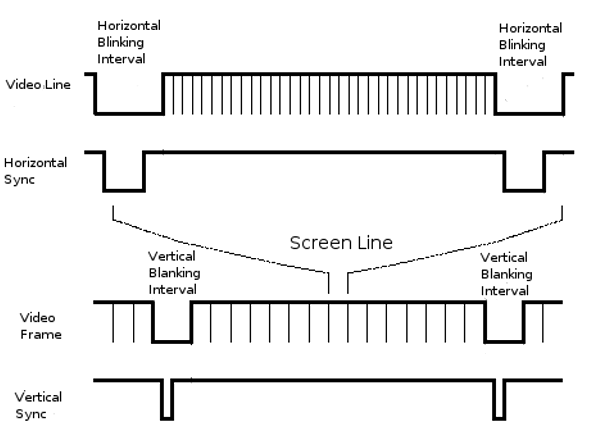
\includegraphics[width=0.7\textwidth]{Grundlagen/vga_timing.png}
	\caption{VGA-Timing, Quelle: \cite{Valcarce2011}}
	\label{fig:vga_timing}
\end{figure}

\subsection{DVI}
Hinter DVI steht der Begriff Digital Visual Interface und stellt ein digitale Schnittstelle zur Grafikanzeige dar. Der DVI Standard wurde 1999 von der DDWG\footnote{Digital Display Working Group} verabschiedet, da der Wunsch nach Leistungsstärkeren Schnittstellen vorhanden war. QXGA-Auflösungen\footnote{QXGA: 2048x1536} sind auf analogem Wege nicht mehr befriedigend erzielbar. Die DVI Schnittstelle beinhaltet neben den Digitalen Signalen zusätzlich analoge VGA Signale, was den Betrieb älterer Monitore und Displays zulässt. Zur digitalen Datenübertragung wird der TMDS\footnote{Transition Minimized Differential Signaling - Differentielle Datenübertragung} Standard verwendet, welcher die 24 Bit Farbinformationen\footnote{24 Bit: je 8 Bit für Rot, Grün und Blau} mittels eines Serializers in serielle Daten umwandelt. Je nach benötigter Bandbreite können drei oder sechs Aderpaare für Pixeldaten verwendet werden. Dies wird Single-Link bzw. Double-Link genannt und es lassen sich dabei max. 3.72 GBit/s\footnote{max. UXGA: 1600x1200@60Hz} bzw. 7.44 GBit/s\footnote{max. WUXGA: 1920x1200@60Hz} übertragen. Um die Paare zuordnen zu können, wird ein weiteres Paar zur Synchronisation verwendet. Um die Übertragung noch effizienter zu gestalten, gibt es die Möglichkeit bei High- sowie Low-Pegel des Taktsignals Daten zu übertragen\footnote{\textit{Double Data Rate}} (\cite{Leunig2002}).

\subsection{HDMI}
Gegeneber der DVI-Schnittstelle bietet die HDMI Schnittstelle dieselben Eigenschaften bezüglich der Videoübertragung verwendet zur ebenfalls TMDS. Hinzu kommt allerdings, dass sowohl Audio als auch Verschlüsselung unterstützt werden. Der Formfaktor der Stecker sind für den Hausgebrauch verkleinert worden. HDMI wurde als normierte Universallösung entwickelt und hat sich als solche etabliert (\cite{Extron2014}). Nahezu jedes neu entwickelte Gerät mit Anzeigemöglichkeit, bietet eine HDMI-Schnittstelle - ebenso embedded Linux Boards wie z.B. bekannte Linux Boards wie Raspberry Pi oder Beagle Bone Black.

\subsection{RGB}
Der RGB-Bus, verwendet für kleine TFT-Panels bis ca. 7", funktioniert prinzipiell analog zur VGA-Schnittstelle, mit dem Unterschied, dass die Datenleitungen komplett digital sind. 
So werden die Signale für Rot, Grün und Blau nicht mehr analog im Bereich von 0V bis +0.7V dargestellt, sondern durch einen üblicherweise acht Bit breiten Bus pro Farbkanal. Die Auflösung pro Farbkanal ist mit 255 Intensitätsstufen gerechnet ausreichend um ein gesamtes Farbspektrum von 16777216 \footnote{16777216 Farben = 2\textasciicircum24} Farben zu erhalten. 
\begin{figure}[htp]
	\centering
	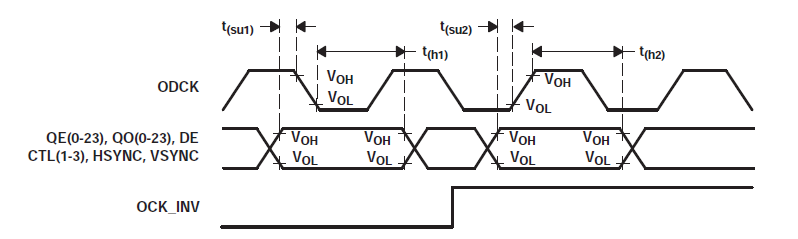
\includegraphics[width=0.8\textwidth]{Grundlagen/rgb_timing.png}
	\caption{RGB-Timing, Quelle: \cite{TI2011}}
	\label{fig:rgb_timing}
\end{figure}
Dieser Farbmodus wird auch RGB888 genannt, da acht Bit für jede Farbe zur Kodierung, insgesamt also 24 Bit, zur Verfügung stehen. Neben dem 24 Bit Modus ist RGB565 noch weit verbreitet, der je fünf Bit für Rot und Blau und sechs Bit für Grün verwendet. Hier ergibt sich ein Farbspektrum von 65536\footnote{65536 = 2\textasciicircum16} Farben. Da digital übertragen wird, ist eine Taktleitung notwendig um die Synchronizität zu ermöglichen. 
Aufgrund der Verbreitung und Mächtigkeit der Schnittstelle besitzen einige Prozessor, wie z.B. der Linuxfähige OMAP3530 von Texas Instruments, eine RGB-Schnittstelle. 
\refa{fig:rgb_timing} zeigt exemplarisch ein Timing-Diagramm der RGB-Schnittstelle des Bausteins TFP-401A von Texas Instruments.
\subsection{LVDS}
Um lange Strecken und große Bildformate übertragen zu können ist der parallele Datentransfer ungeeignet, da bei schnellem Takt z.B. das Übersprechen zu groß wird und das Signal schneller gestört wird. Deshalb ist die Praktik beliebt, große Datenmengen über eine differentielle Verbindung wie z.B. LVDS\footnote{LVDS: Low Voltage Differential Signaling} zu übertragen. Die physikalische Funktionsweise der LVDS Leitung liegt darin, dass zweimal dasselbe Signal übertragen wird - mit positiver Spannung und mit negativer Spannung. Wirkt nun von außen eine Störung auf die LVDS Leitung, werden beide Leitungen - positive wie auch die negative - gleichermaßen gestört. Durch das Zusammenführen beider Signale am Ende, kompensieren sich diese Störungen im Idealfall zu Null. Wie auch LVDS arbeitet das zuvor genannte TMDS ähnlich, da es sich hierbei auch um eine differentielle Übertragungsart handelt. Der Unterschied liegt in der Verwendung. TMDS wird oft eingesetzt, sobald das Signal das Gerät verlässt - z.B. Desktop-Bildschirm mit Anschlusskabel. Befindet sich das Anzeigegerät allerdings im selben Gehäuse, so wird oft LVDS eingesetzt. Neben Bilddaten ist es natürlich auch möglich andere Nutzdaten wie z.B. Sensordaten zu übertragen. 
Aufgrund der hohen Geschwindigkeit und geringen Fehlerrate werden differentiellen Übertragungen werden gerne für Displays angewendet.
\subsection{8080-Interface}
Das 8080-Interface ist eine antike Schnittstelle ursprünglich von Intel 8080 Prozessor. Sie wird bis heute verwendet, um Speicher, kleine TFT-Displays oder andere Bausteine mit einem Mikrocontroller zu betreiben. Eckdaten des 8080-Interface sind sowohl der Datenbus selbst als auch der Adressbus mit z.B. acht, 16 oder 32 Bit, je eine eine Leitung für Read-Enable, Write-Enable und Chip-Select. Durch die Verwendung der Chip-Select Leitungen ist es möglich mehrere Teilnehmer am selben Bus zu betreiben. Alle Teilnehmer, deren Chip-Leitung nicht aktiv ist, verhalten sich für andere Busteilnehmer unsichtbar. Erst mit Zuweisung der Chip-Selects werden diese sichtbar und übernehmen den Bus. Ein Hostsystem steuert als sog. Master die am Bus hängenden Slaves. Moechte das Hostsystem von einem Slave Daten lesen, wird ein Lesezyklus initiiert, der die Chip-Select Leitung aktiviert, die gewünschte Adresse an den Bus anlegt, die Read-Enable Leitung aktiviert und nach einer festgelegten Zeit diese wieder deaktiviert. Der Slave legt die gewünschten Daten auf den Datenbus und der Host kann diese Daten korrekt lesen. Analog dazu funktioniert der Schreibzyklus ähnlich. 
\refa{fig:8080_timing} zeigt das Timing Diagramm eines Schreib- und Lesezyklus des Displaycontrollers SSD1289. Das Signal D/C wird verwendet um zu unterscheiden, ob ein Daten oder ein Kommando auf dem Bus anliegen. Dazu kann beispielsweise eine Adressleitung des 8080-Bus verwendet werden. CS stellt das Chip-Select dar. WR und RD beziehen sich auf Write- bzw. Read-Enable. D0-D17 sind 18 Datenbits des Bus (\cite{SSD2007}). 

\begin{figure}[htp]
	\centering
	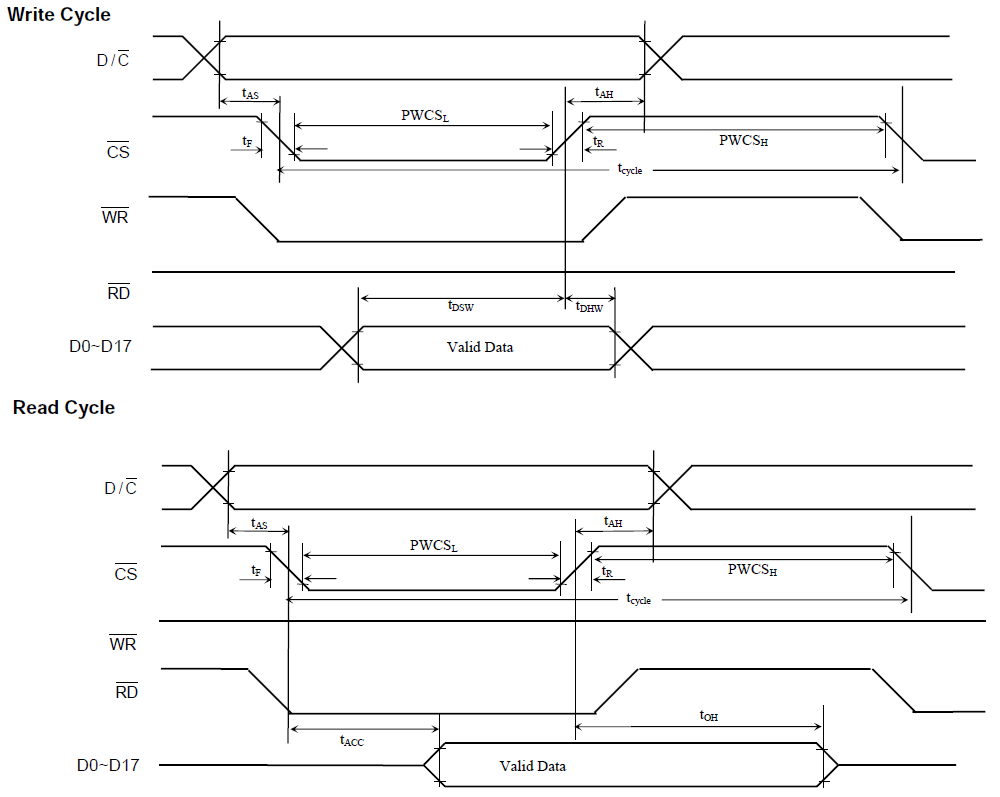
\includegraphics[width=1.0\textwidth]{Grundlagen/8080_timing.png}
	\caption{8080-Timing des SSD1289, Quelle: \cite{SSD2007}}
	\label{fig:8080_timing}
\end{figure}


Viele Mikrocontroller besitzen bereits ein 8080-Interface dediziert in Hardware - allerdings nicht alle. Als Ersatz kann das Protokoll mit GPIO\footnote{GPIO: General Purpose In/Output} in Software implementiert werden. Dies ist allerdings wesentlich langsamer als eine Lösung, die bereits in Hardware läuft, da GPIO-Pins nicht dafür geschaffen sind, sich mit schneller Frequenz schalten zu lassen.
\clearpage

\subsection{Bewertung der Video-Schnittstellen}
\label{cha:bewertung_video}
Nachdem nun die wichtigsten Schnittstellen dargestellt wurden, werden diese im Folgenden mit dem Fokus auf die Masterareit hinsichtlich der Relevanz bewertet.
Da die VGA-Schnittstelle antik und obsolet ist, spielt sie heutzutage nur noch eine geringe Rolle. Insbesondere im Bereich der embedded Systeme wird sie kaum verwendet. Für die Masterarbeit ist die VGA-Schnittstelle uninteressant, da diese von keiner, in der Masterarbeit behandelten, Hardware verwendet wird. Jedoch wurde diese eingangs behandelt, da diese den Übergang zum digitalen RGB-Bus schafft.\\
Die DVI- und HDMI-Schnittstellen, welche für den Bereich der Videoanzeige praktisch identisch sind, nehmen jedoch einen hohen Stellenwert in der Masterarbeit ein. Im zweiten Teil der Arbeit wird eine Hardware entwickelt, welche als Eingangssignale die TMDS der DVI-/HDMI-Schnittstelle nutzt. 
Ebenso spielen die RGB-Schnittstelle und LVDS eine große Rolle\todo{große Rolle: umschreiben}, da an diesen Schnittstellen der entwickelten Hardware TFT-Panels angeschlossen werden. \\
Neben den reinen Video-Schnittstellen weist das beschriebene 8080-Interface, das ursprünglich nicht zur Bildübertragung gedacht war, ein hohes Potential auf und besitzt für den ersten Teil der Masterarbeit hohen Stellenwert. Gerade im embedded Bereich besitzt diese Schnittstelle nach wie vor einen hohen Stellenwert, da vor allem kleine Displays damit hinreichend schnell und effizient betrieben werden können. \reft{tab:interface_vergleich} zeigt nochmals eine kurze Übersicht der Relevanz der einzelnen Schnittstellen für die Masterarbeit.

\begin{table}[h]
\begin{tabular}{|c|c|c|}\hline
   \textbf{Schnittstelle} 	& \textbf{Relevanz für Masterarbeit} 	& \textbf{Verwendung in der Masterarbeit}	\\ \hline
   VGA 						& keine  								& - 	 									\\ \hline
   DVI 						& mittel 								& Teil B 									\\ \hline
   HDMI						& hoch 									& Teil B 									\\ \hline
   RGB 						& hoch 									& Teil B 									\\ \hline
   LVDS 					& hoch									& Teil B 									\\ \hline
   8080-Interface 			& hoch 									& Teil A 									\\ \hline
\end{tabular}
\caption{Relevanz der Display-Schnittstellen für die Masterarbeit}
\label{tab:interface_vergleich}
\end{table}

\section{Betrachtete Embedded Linux Boards}
\label{cha:betrachtete_linux_boards}
In diesem Abschnitt werden die verwendeten Linux-Boards dargestellt, verglichen und hinsichtlich der Verwendbarkeit in der Masterarbeit bewertet. Da sich die Masterarbeit in zwei Teile gliedert, wird für beide Anwendungsfaelle ein typisches Linux-Board hergezogen, welches den Anforderungen gerecht werden muss, eine billige und effiziente Anzeige zu gestatten.
\subsection{Raspberry Pi}
\label{cha:raspberry}
Am wohl bekanntesten und mit einer riesigen Community hinter dem Projekt ist der Raspberry Pi von der Raspberry Pi Foundation \footnote{\url{http://www.raspberrypi.org}}. Um die wichtigsten Eckdaten des Einplatinenrechners im Checkkartenformat zu nennen, besitzt er in der Ausfuehrung Model B einen ARM11-Core (Broadcom BCM2835), 512 Megabyte SDRAM, eine Broadcom VideoCore IV GPU sowie diverse Schnittstellen wie HDMI, USB 2.0, UART\footnote{UART: Universal Asynchronous Receiver Transmitter - RS2332}, SPI\footnote{SPI: Serial Peripheral Interface - 4 Draht Bus}, I2C\footnote{I2C: Inter Integrated Circuit - 2 Draht Bus} sowie GPIO-Pins\footnote{GPIO: General Purpose Input Output}.\\
Der erschwingliche Preis macht den Raspberry Pi attraktiv und zieht die Community an, da man für rund 40 Euro einen kompletten Rechner bekommt. \\
\begin{tabular}{|c|c|}\hline
   Lehrstuhl & Professor \\ \hline
   BWL & Maier \\ \hline
   MB & M"uller \\ \hline
   Jura & Schmidt \\ \hline
 \end{tabular}


\subsection{Gnublin Extended}
\label{cha:gnublin_extended}
\todo{8080-Interface in SRAM erwaehnen!}


\subsection{Bewertung der Linux-Boards}
\label{cha:bewertung_linux_boards}
